\begin{theorem}\label{thm:change_of_basis} For $\tpi\in\tilde\Pi_{2(r),k}$ whose unbarred entries have multiplicity given by $\bfa\in W_{r,k}$, write \[\omega(\tpi)=\frac{m(\tpi)!}{\abs{\SG_\bfa}}\prod_{\tB\in\tpi}m(\tB|_{\ovb{k}})!.\] Then the map \begin{align*}
    \varphi:\tilde{P}_{r,k}(x)&\to\MP_{r,k}(x)\\
    \OO_\tpi&\mapsto \omega(\tpi)\XX_\tpi
\end{align*} where $\{\XX_\tpi:\tpi\in\tilde\Pi_{2(r),k}\}$ is the orbit basis of Orellana and Zabrocki is an isomorphism of algebras.
\end{theorem}

Because each $\omega(\tpi)$ is nonzero, it is clear that this map is an isomorphism of vector spaces--the remainder of this section is devoted to proving that it respects the multiplication. First, we observe that such an isomorphism gives us the following change-of-basis formula from Orellana and Zabrocki's orbit basis to the diagram-like basis:

\begin{align*}
    \DD_\tpi&=\varphi(s_\bfa L_\pi s_\bfb)\\
            &=\sum_{\tnu\leq\tpi} c_{\tnu,\tpi}\omega(\tnu)\XX_\tnu
\end{align*} where for a fixed $\pi$ such that $\kappa_{\bfa,\bfb}(\pi)=\tpi$, $c_{\tnu,\tpi}$ is the number of $\nu\leq\pi$ such that $\kappa_{\bfa,\bfb}(\nu)=\tnu$.

\begin{exam} We expand the following diagram-like basis element in the orbit basis of Orellana and Zabrocki:
    \newcommand{\subdiag}[1]{\hspace{-.08in}\begin{tabular}{c}
    \begin{tikzpicture}[xscale=.25,yscale=.25,line width=1pt] 
        \foreach \i in {1,2,3,4}  { \path (\i,1.25) coordinate (T\i); \path (\i,.25) coordinate (B\i);} 
        \filldraw[fill= black!12,draw=black!12,line width=4pt]  (T1) -- (T4) -- (B4) -- (B1) -- (T1);
        #1
        \colortop{1,2,3,4}{black}
        \colorbot{1,2,3,4}{black}
    \end{tikzpicture}
\end{tabular}}

\newcommand{\submultidiag}[1]{\hspace{-.08in}\begin{tabular}{c}
    \begin{tikzpicture}[xscale=.25,yscale=.25,line width=1pt] 
        \foreach \i in {1,2,3,4}  { \path (\i,1.25) coordinate (T\i); \path (\i,.25) coordinate (B\i);} 
        \filldraw[fill= black!12,draw=black!12,line width=4pt]  (T1) -- (T4) -- (B4) -- (B1) -- (T1);
        #1
        \colortop{1,2}{c1}
        \colortop{3,4}{c2}
        \colorbot{1,2,3}{c1}
        \colorbot{4}{c2}
    \end{tikzpicture}
\end{tabular}}


\begin{align*}
    \DD_{\submultidiag{\draw[black] (T1)--(B1);\draw[black] (T2)--(B2);\draw[black] (T3)--(T4)--(B4)--(B3)--(T3);}}&=s_{(2,2)}\LL_{\subdiag{\draw[black] (T1)--(B1);\draw[black] (T2)--(B2);\draw[black] (T3)--(T4)--(B4)--(B3)--(T3);}}s_{(3,1)}\\
    \hspace{-.1in}&=s_{(2,2)}\Big(
    \TT_{\subdiag{\draw[black] (T1)--(B1);\draw[black] (T2)--(B2);\draw[black] (T3)--(T4)--(B4)--(B3)--(T3);}}
    \hspace{-.1in}+\TT_{\subdiag{\draw[black] (T1)--(B1)--(B2)--(T2)--(T1);\draw[black] (T3)--(T4)--(B4)--(B3)--(T3);}}
    \hspace{-.1in}+\TT_{\subdiag{\draw[black] (T1)--(B1);\draw[black] (T2)--(T4)--(B4)--(B2)--(T2);}}
    \hspace{-.1in}+\TT_{\subdiag{\draw[black] (T1)  .. controls +(0,-.4) and +(0,-.4) .. (T3) -- (T4) -- (B4) -- (B3) .. controls +(0,+.4) and +(0,+.4) .. (B1) -- (T1);\draw[black] (T2) -- (B2);}}
    \hspace{-.1in}+\TT_{\subdiag{\draw[black] (T1)--(T4)--(B4)--(B1)--(T1);}}\hspace{-.1in}\Big)s_{(3,1)}
\end{align*}
\begin{align*}
    \DD_{\submultidiag{\draw[black] (T1)--(B1);\draw[black] (T2)--(B2);\draw[black] (T3)--(T4)--(B4)--(B3)--(T3);}}&=\hspace{.35in}\OO_{\submultidiag{\draw[black] (T1)--(B1);\draw[black] (T2)--(B2);\draw[black] (T3)--(T4)--(B4)--(B3)--(T3);}}
    \hspace{-.1in}+\hspace{.35in}\OO_{\submultidiag{\draw[black] (T1)--(B1)--(B2)--(T2)--(T1);\draw[black] (T3)--(T4)--(B4)--(B3)--(T3);}}
    \hspace{-.1in}+\hspace{.3in}2\OO_{\submultidiag{\draw[black] (T1)--(B1);\draw[black] (T2)--(T4)--(B4)--(B2)--(T2);}}
    \hspace{-.1in}+\hspace{.35in}\OO_{\submultidiag{\draw[black] (T1)--(T4)--(B4)--(B1)--(T1);}}\\
    &\mapsto\omega(\tpi_1)\XX_{\submultidiag{\draw[black] (T1)--(B1);\draw[black] (T2)--(B2);\draw[black] (T3)--(T4)--(B4)--(B3)--(T3);}}
    \hspace{-.1in}+\omega(\tpi_2)\XX_{\submultidiag{\draw[black] (T1)--(B1)--(B2)--(T2)--(T1);\draw[black] (T3)--(T4)--(B4)--(B3)--(T3);}}
    \hspace{-.1in}+2\omega(\tpi_3)\XX_{\submultidiag{\draw[black] (T1)--(B1);\draw[black] (T2)--(T4)--(B4)--(B2)--(T2);}}
    \hspace{-.1in}+\omega(\tpi_4)\XX_{\submultidiag{\draw[black] (T1)--(T4)--(B4)--(B1)--(T1);}}
    \\
    &=\hspace{.23in}\frac{2!}{3!}\XX_{\submultidiag{\draw[black] (T1)--(B1);\draw[black] (T2)--(B2);\draw[black] (T3)--(T4)--(B4)--(B3)--(T3);}}
    \hspace{-.1in}+\hspace{.2in}\frac{2!}{3!}\XX_{\submultidiag{\draw[black] (T1)--(B1)--(B2)--(T2)--(T1);\draw[black] (T3)--(T4)--(B4)--(B3)--(T3);}}
    \hspace{-.1in}+\hspace{.2in}2\frac{2!}{3!}\XX_{\submultidiag{\draw[black] (T1)--(B1);\draw[black] (T2)--(T4)--(B4)--(B2)--(T2);}}
    \hspace{-.1in}+\hspace{.21in}\frac{3!}{3!}\XX_{\submultidiag{\draw[black] (T1)--(T4)--(B4)--(B1)--(T1);}}\\
    &=\hspace{.26in}\frac13\XX_{\submultidiag{\draw[black] (T1)--(B1);\draw[black] (T2)--(B2);\draw[black] (T3)--(T4)--(B4)--(B3)--(T3);}}
    \hspace{-.1in}+\hspace{.24in}\frac13\XX_{\submultidiag{\draw[black] (T1)--(B1)--(B2)--(T2)--(T1);\draw[black] (T3)--(T4)--(B4)--(B3)--(T3);}}
    \hspace{-.1in}+\hspace{.32in}\frac23\XX_{\submultidiag{\draw[black] (T1)--(B1);\draw[black] (T2)--(T4)--(B4)--(B2)--(T2);}}
    \hspace{-.1in}+\hspace{.34in}\XX_{\submultidiag{\draw[black] (T1)--(T4)--(B4)--(B1)--(T1);}}
\end{align*}
\end{exam}

\subsection{Preliminary definitions and enumerative results}

The product formula for the orbit basis $\{\TT_\pi:\pi\in\Pi_{2(r)}\}$ for $P_r(x)$ uses set partitions that include unbarred, barred, and double-barred elements. To that end, we make the following definitions. For $\pi,\nu\in\Pi_{2(r)}$, write $\Gamma^\pi_\nu$ for the set of set partitions $\gamma$ of $[r]\cup\ovb{r}\cup\ovovb{r}$ such that $\gamma|_{[r]\cup\ovb{r}}=\pi$ and $\gamma|_{\ovb{r}\cup\ovovb{r}}=\ov\nu$ where $\ov\nu$ is the result of adding a bar to each element in $\nu$. For such a $\gamma$, write $\beta_\gamma=\{S\in\gamma:\forall i\in S, i\in\ovb{r}\}$ for the set of blocks of $\gamma$ containing only barred numbers. Write \[b_\gamma(x)=(x-\ell(\gamma|_{[r]\cup\ovovb{r}}))_{\ell(\beta_\gamma)}\]  where $(a)_n=a(a-1)\cdots(a-n+1)$. The product formula for the orbit basis is

\begin{align*}
    \TT_\pi \TT_\nu&=\sum_{\gamma\in\Gamma^\pi_\nu}b_\gamma(x)\TT_\gamma
\end{align*} where the $\gamma$ in the subscript is understood to be an element of $\Pi_{2(r)}$ by taking the restriction $\gamma|_{[r]\cup\ovovb{r}}$ and removing a bar from each double-barred entry (see Theorem 4.14 of \cite{Benkart2019PartitionAA} for details).

For the orbit basis $\{\XX_\tpi:\tpi\in\tilde\Pi_{2(r),k}\}$ of $\MP_{r,k}(x)$ we make similar definitions. For $\tpi,\tnu\in\tilde\Pi_{2(r),k}$, write $\tilde\Gamma^\tpi_\tnu$ for the set of multiset partitions $\tgamma$ with $r$ elements each from $[k]$, $\ovb{k}$, and $\ovovb{k}$ such that $\tgamma|_{[k]\cup\ovb{k}}=\tpi$ and $\tgamma|_{\ovb{k}\cup\ovovb{k}}=\ov\tnu$. For such a $\tgamma$, write $\beta_\tgamma=\multi{\tS\in\tgamma:\forall i\in \tS, i\in\ovb{k}}$. Finally, write \begin{align*}
    \tilde{b}_\tgamma(x)&=\frac{(x-\ell(\tgamma|_{[k]\cup\ovovb{k}}))_{\ell(\beta_\tgamma)}}{m(\beta_\tgamma)!}\\
    a_\tgamma&=\prod_{\substack{\tS\in\tgamma|_{[k]\cup\ovovb{k}}\\\text{distinct}}}\frac{\ell(\tgamma_\tS)!}{m(\tgamma_\tS)!}
\end{align*} where $\tgamma_\tS=\multi{\tT\in\tgamma:\tT|_{[k]\cup\ovovb{k}}=\tS}$. Then, the product for the orbit basis of $\MP_{r,k}(x)$ is given by \begin{align*}
    \XX_\tpi \XX_\tnu &=\sum_{\tgamma\in\tilde\Gamma^\tpi_\tnu} a_\tgamma \tilde{b}_\tgamma(x) \XX_\tgamma
\end{align*} where the $\tgamma$ in the subscript is understood to be an element of $\tilde{\Pi}_{2r,k}$ by taking the restriction $\gamma|_{[k]\cup\ovovb{k}}$ and removing a bar from each double-barred entry (see Section 3 of \cite{orellana2020howe} for details).

To handle these set and multiset partitions on three alphabets combinatorially, we will want to extend the notation of our painting function $\kappa_{\bfa,\bfb}$ to them. In particular, $\kappa_{\bfa,\bfb,\bfc}(\gamma)$ will be the result of replacing the unbarred, barred, and double-barred elements according to $\bfa,\bfb$, and $\bfc$ respectively. It will be useful later to write $\Gamma_\nu^\pi(\tmu)$ for the set of $\gamma\in\Gamma_\nu^\pi$ such that $\kappa_{\bfa,\bfb,\bfc}(\gamma)=\tmu$.

For $\pi,\nu\in\Pi_{2(r)}$ with $\pi|_{\ovb{r}}=\ov\nu|_{\ov r}$, let $\pi\ast\nu\in\Gamma^\pi_\nu$ be the set partition obtained by placing the diagram of $\pi$ atop the diagram of $\nu$ and identifying the corresponding vertices in the center. This set partition plays a central role because any $\gamma\in\Gamma^\pi_\nu$ only differs from $\pi\ast\nu$ by connecting some blocks on the very top and very bottom. That is, if we denote by \defn{$\Break(\gamma)$} the result of splitting each block of $\gamma$ that does not contain a vertex in the middle row of the diagram into its restriction to $[r]$ and restriction to $\ovb{r}$, then $\gamma\in\Gamma^\pi_\nu$ if and only if $\Break(\gamma)=\pi\ast\nu$.

\begin{exam} We compute $\Break(\gamma)$ of a set partition $\gamma$ of $[6]\cup\ovb{6}\cup\ovovb{6}$.
    \begin{align*}
        \gamma=\begin{array}{c}
            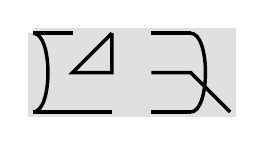
\begin{tikzpicture}[xscale=.5,yscale=.5,line width=1.25pt] 
                \foreach \i in {1,2,3,4,5,6}  { \path (\i,1.25) coordinate (T\i); \path (\i,.25) coordinate (M\i); \path (\i,-.75) coordinate (B\i); } 
                \filldraw[fill= black!12,draw=black!12,line width=4pt]  (T1) -- (T6) -- (B6) -- (B1) -- (T1);
                \draw[black] (T1) .. controls +(+0.50,0) and +(+0.50,0) .. (B1);
                \draw[black] (T1) -- (T2);
                \draw[black] (B1) -- (B2) -- (B3);
                \draw[black] (T3) -- (M3) -- (M2) -- (T3);
                \draw[black] (T4) -- (T5);
                \draw[black] (T5) .. controls +(+0.50,0) and +(+0.50,0) .. (B5);
                \draw[black] (B4) -- (B5);
                \draw[black] (M4) -- (M5) -- (B6);
                \colortop{1,2,3,4,5,6}{black}
                \colormid{1,2,3,4,5,6}{black}
                \colorbot{1,2,3,4,5,6}{black}
            \end{tikzpicture}
        \end{array} && \Break(\gamma)= \begin{array}{c}
            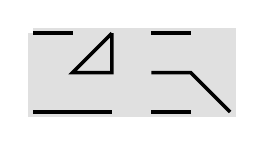
\begin{tikzpicture}[xscale=.5,yscale=.5,line width=1.25pt] 
                \foreach \i in {1,2,3,4,5,6}  { \path (\i,1.25) coordinate (T\i); \path (\i,.25) coordinate (M\i); \path (\i,-.75) coordinate (B\i); } 
                \filldraw[fill= black!12,draw=black!12,line width=4pt]  (T1) -- (T6) -- (B6) -- (B1) -- (T1);
                \draw[black] (T1) -- (T2);
                \draw[black] (B1) -- (B2) -- (B3);
                \draw[black] (T3) -- (M3) -- (M2) -- (T3);
                \draw[black] (T4) -- (T5);
                \draw[black] (B4) -- (B5);
                \draw[black] (M4) -- (M5) -- (B6);
                \colortop{1,2,3,4,5,6}{black}
                \colormid{1,2,3,4,5,6}{black}
                \colorbot{1,2,3,4,5,6}{black}
            \end{tikzpicture}
        \end{array}
    \end{align*}
\end{exam}

To analyze the orbit basis of $\MP_{r,k}(x)$, we want to investigate how $\pi\ast\nu$ acts when $\nu$ is acted upon by some permutation. This inspires the definition of several subgroups of permutations. For $\rho$ a set partition of $[r]$ and $\bfa\in W_{r,k}$, define \begin{align*}
    \SG_\bfa^\rho=\{\sigma\in\SG_\bfa:\sigma.\rho=\rho\}
\end{align*} where the action $\sigma.\rho$ applies $\sigma$ to each element of each block of $\rho$. This subgroup factors as a semidirect product \begin{align*}
    \SG_\bfa^\rho=X_\bfa^\rho Y_\bfa^\rho
\end{align*} where the permutations in $X_\bfa^\rho$ permute whole blocks and the permutations in $Y_\bfa^\rho$ permute only within blocks of $\rho$.

\begin{exam} For clarity, we illustrate the above factorization in the case that all elements are the same color (where the corresponding young subgroup $\SG_{(r)}$ is equal to the full symmetric group $\SG_r$). The permutation \[\sigma=(3\,4)(1\,5)(2\,6)(8)(7\,9)\] fixes the set partition $\rho=\{\{1,2,4\},\{3,5,6\},\{8\},\{7,9\}\}$ and hence $\sigma\in \SG_{(r)}^\rho$. It then factors as $\sigma=\sigma_X\sigma_Y$ where \[\sigma_X=(1\,4\,2)(3\,5\,6)(7\,9)\] permutes elements within each block and \[\sigma_Y=(1\,3)(2\,5)(4\,6)\] swaps the two blocks of $\rho$ of size three. 
\end{exam}

Given $\pi\in\Pi_{2(r)}$, consider the subgroup $A_{\bfa,\bfb}^\pi$ of $X_\bfb^{\pi|_{\ovb{r}}}$ that only permutes blocks in $\pi|_{\ovb{r}}$ if they are part of blocks of $\pi$ that are painted identically by $\kappa_{\bfa,\bfb}$ (see Example \ref{ex:kappa}). Let $B_{\bfa,\bfb}^\nu$ be the analogous subgroup of $X_\bfb^{\nu|_{\ovb{r}}}$ for the restrictions to the top. More precisely,
\begin{align*}
    A^\pi_{\bfa,\bfb}&=\{\sigma\in X_\bfb^{\pi|_{\ovb{r}}}:\forall S,T\in\pi, S|_{\ovb{r}}=\sigma(T|_{\ovb{r}})\implies \kappa_{\bfa,\bfb}(S)=\kappa_{\bfa,\bfb}(T)\}\\
    B^\nu_{\bfb,\bfc}&=\{\sigma\in X_\bfb^{\nu|_{[r]}}:\forall S,T\in\nu, S|_{[r]}=\sigma(T|_{[r]})\implies \kappa_{\bfb,\bfc}(S)=\kappa_{\bfb,\bfc}(T)\}
\end{align*}

Put another way, these permutations $\sigma$ of the blocks in the middle row of $\pi\ast\nu$ do not change the resulting multiset partition. That is, $\kappa_{\bfa,\bfb,\bfc}(\pi\ast\nu)=\kappa_{\bfa,\bfb,\bfc}(\pi\ast\sigma.\nu)$ for $\sigma\in A_{\bfa,\bfb}^\pi$ or $\sigma\in B_{\bfb,\bfc}^\nu$.

Finally, we collect up formulas for the sizes of these subgroups. To that end, it will be useful to consider the following multiset partitions obtained by restricting to particular blocks.

\begin{align*}
    \tpi_+&=\{\tS\in\tpi:\forall i\in S,i\in[k]\}\\
    \tpi_-&=\{\tS\in\tpi:\forall i\in S,i\in\ovb{k}\}\\
    \tgamma_\pm&=\{\tS\in\tpi:\forall i\in S,i\in[k]\cup\ovovb{k}\}
\end{align*}

We think of $\tpi_+$ (resp. $\tpi_-$) as the blocks contained entirely in the top (resp. bottom) of $\tpi$ and $\tgamma_\pm$ as the blocks of $\tgamma$ that have no vertex in the middle row.

\begin{lemma}\label{lem:subgroup_sizes}
    Let $\bfa,\bfb,\bfc\in W_{r,k}$, $\pi,\nu\in\Pi_{2(r)}$, $\tpi=\kappa_{\bfa,\bfb}(\pi),$ and $\tnu=\kappa_{\bfb,\bfc}(\nu)$. Then, the subgroups defined above have sizes given by the following.

    \begin{align*}
        \begin{array}{ccc}
            \abs{X^\rho_\bfa}=m(\kappa_\bfa(\rho))! & \hspace{.5in} & \abs{Y^\rho_\bfa}=\prod_{\tB\in\tpi}m(\tB|_{\ovb{k}})! \\
            \abs{A^\pi_{\bfa,\bfb}}=\frac{m(\tpi)!}{m(\tpi_+)!} & & \abs{B^\nu_{\bfb,\bfc}}=\frac{m(\tnu)!}{m(\tnu_-)!}
        \end{array}
    \end{align*}

    Furthermore, for any $\tgamma\in\tilde\Gamma^\tpi_\tnu$, the size of the intersection of $A^\pi_{\bfa,\bfb}$ and $B^\nu_{\bfb,\bfc}$ is given by \begin{align*}
        \abs{A^\pi_{\bfa,\bfb}\cap B^\nu_{\bfb,\bfc}}&=\frac{m(\tgamma)!}{m(\tgamma_\pm)!}.
    \end{align*}
\end{lemma}

\begin{proof}
    The equalities in the first row are clear. The next two follow from the observation that the only blocks of $\tpi$ that contribute to $A_{\bfa,\bfb}^\pi$ are the ones that touch the bottom, so we cancel out the contribution of those contained entirely in the top.

    For the last equality, we can think of $A_{\bfa,\bfb}^\pi\cap B^\nu_{\bfb,\bfc}$ as the permutations of the vertices in the middle row of $\pi\ast\nu$ that only permute blocks that are the restrictions of blocks painted the same in $\kappa_{\bfa,\bfb,\bfc}(\pi\ast\nu)$. The number of such permutations is $\frac{m(\kappa_{\bfa,\bfb,\bfc}(\pi\ast\nu))!}{m(\kappa_{\bfa,\bfb,\bfc}(\pi\ast\nu)_\pm)!}$. Because $\tgamma$ only differs from $\kappa_{\bfa,\bfb,\bfc}(\pi\ast\nu)$ by blocks that do not touch the center (whose contributions are all canceled) we can make the substitution of $\tgamma$ for $\kappa_{\bfa,\bfb,\bfc}(\pi\ast\nu)$.
\end{proof}



\subsection{Proof of the isomorphism}

\begin{proof}[Proof of Theorem \ref{thm:change_of_basis}]
    Let $\tpi,\tnu\in\tilde\Pi_{2(r)}$ and let $\bfa,\bfb,\bfb',\bfc\in W_{r,k}$ be such that there exist $\pi,\nu\in\Pi_{2(r)}$ so that $\kappa_{\bfa,\bfb}(\pi)=\tpi$ and $\kappa_{\bfb',\bfc}(\nu)=\tnu$. Note that when $\bfb\neq\bfb'$, we have $\OO_\tpi\OO_\tnu=0$ and $\XX_\tpi \XX_\tnu=0$, so we need only address the case when $\bfb=\bfb'$:

    \begin{align*}
        \OO_\tpi\OO_\tnu&=\frac{1}{\abs{\SG_\bfb}}\sum_{\sigma\in\SG_\bfb}s_\bfa\TT_\pi\TT_{\sigma.\nu}s_\bfc\\
        &=\frac{1}{\abs{\SG_\bfb}}\sum_{\sigma\in\SG_\bfb}\sum_{\gamma\in\Gamma^\pi_{\sigma.\nu}} b_\gamma(x) s_\bfa \TT_\gamma s_\bfb\\
        \intertext{To simplify notation, we will write $\tgamma=\kappa_{\bfa,\bfb,\bfc}(\gamma)$. Note that $b_\gamma(x)=\tilde{b}_{\tgamma}(x)m(\beta_\tgamma)!$, so we can rewrite the expression as follows.}
        \OO_\tpi\OO_\tnu&=\frac{1}{\abs{\SG_\bfb}}\sum_{\sigma\in\SG_\bfb}\sum_{\gamma\in\Gamma^\pi_{\sigma.\nu}} \tilde{b}_\tgamma(x)m(\beta_\tgamma)! \OO_{\tgamma}\\
        \intertext{We then partition the sum over the possible multiset partitions $\tmu$ that could arise from $\gamma$ in this sum, noting that $\kappa_{\bfb,\bfc}(\sigma.\nu)=\tnu$, and then we swap the order of summation to obtain}
        \OO_\tpi\OO_\tnu&=\frac{1}{\abs{\SG_\bfb}}\sum_{\tmu\in\tilde\Gamma_{\tnu}^\tpi} \tilde{b}_\tmu(x)m(\beta_\tmu)!\bigg(\sum_{\sigma\in\SG_\bfb}\sum_{\substack{\gamma\in\Gamma^\pi_{\sigma.\nu}\\\tgamma=\tmu}}1\bigg)\OO_\tmu\\
        &=\frac{1}{\abs{\SG_\bfb}}\sum_{\tmu\in\tilde\Gamma_{\tnu}^\tpi} \tilde{b}_\tmu(x)m(\beta_\tmu)!\bigg(\sum_{\sigma\in\SG_\bfb}\abs{\Gamma^\pi_{\sigma.\nu}(\tmu)}\bigg)\OO_\tmu.
    \end{align*}
    \begin{align}
        \intertext{Recall that $\varphi(\OO_\tpi)=\omega(\tpi)X_\tpi$. Applying $\varphi$ to both sides of the above equation and writing $\varphi(\OO_\tpi\OO_\tnu)|_{\XX_\ttau}$ for the coefficient of $\XX_\ttau$ in $\varphi(\OO_\tpi\OO_\tnu)$ then yields}
        \varphi(\OO_\tpi\OO_\tnu)|_{\XX_\ttau}&=\frac{\omega(\ttau)}{\abs{\SG_\bfb}}\sum_{\substack{\tmu\in\Gamma^\tpi_\tnu\\\tmu|_{[k]\cup\ovovb{k}}=\ttau}}\tilde{b}_\tmu(x)m(\beta_\tmu)!\bigg(\sum_{\sigma\in\SG_\bfb}\abs{\Gamma^\pi_{\sigma.\nu}(\tmu)}\bigg).\label{eq:phi}\\
        \intertext{We now compare this to the same coefficient in $\varphi(\OO_\tpi)\varphi(\OO_\tnu)$:}
        \varphi(\OO_\tpi)\varphi(\OO_\tnu)|_{\XX_\ttau}&=\omega(\tpi)\omega(\tnu)\sum_{\substack{\tmu\in\tilde\Gamma^\tpi_\tnu\\\tmu|_{[k]\cup\ovovb{k}=\ttau}}}a_\tmu \tilde{b}_\tmu(x)\label{eq:phiphi}
    \end{align}

    The goal is now to show that the rather unpleasant expressions given in Equation \ref{eq:phi} for $\varphi(\OO_\tpi\OO_\tnu)$ and Equation \ref{eq:phiphi} for $\varphi(\OO_\tpi)\varphi(\OO_\tnu)$ are equal. We will leverage their similarities---namely that they sum over the same objects and each include a factor of $\tilde{b}_\tmu(x)$ in each summand---to simplify the task. It would suffice to show the following equality:

    \begin{align*}
        \frac{\omega(\ttau)}{\abs{\SG_\bfb}}m(\beta_\tmu)!\bigg(\sum_{\sigma\in\SG_\bfb}\abs{\Gamma^\pi_{\sigma.\nu}(\tmu)}\bigg)&=\omega(\tpi)\omega(\tnu)a_\tmu
    \end{align*}

    By using the definition of $\omega(\tpi)$ and noticing that $\ttau|_{\ovb{k}}=\tnu|_{\ovb{k}}$, we are able to rearrange the above equality to

    \begin{align*}
        \sum_{\sigma\in\SG_\bfb}\abs{\Gamma^\pi_{\sigma.\nu}(\tmu)}&=a_\tmu\frac{m(\tpi)!m(\tnu)!}{m(\ttau)!m(\beta_\tmu)!}\prod_{\tB\in\tpi}m(\tB|_{\ovb{k}})!.
    \end{align*}
    Then using the formulas in Lemma \ref{lem:subgroup_sizes} for the sizes of the subgroups, we rewrite the right-hand side to obtain
    \begin{align*}
        \sum_{\sigma\in\SG_\bfb}\abs{\Gamma^\pi_{\sigma.\nu}(\tmu)}&=a_\tmu\frac{m(\tpi_+)!m(\tnu_-)!}{m(\ttau)!m(\beta_\tmu)!}\frac{m(\tmu)!}{m(\tmu_\pm)!}\frac{\abs{A^\pi_{\bfa,\bfb}}\abs{B^\nu_{\bfb,\bfc}}\abs{Y_\bfb^{\pi|_{\ovb{r}}}}}{\abs{A_{\bfa,\bfb}^\pi\cap B_{\bfb,\bfc}^\nu}}\\
        &=a_\tmu\frac{m(\tpi_+)!m(\tnu_-)!}{m(\ttau)!m(\beta_\tmu)!}\frac{m(\tmu)!}{m(\tmu_\pm)!}\abs{A_{\bfa,\bfb}^\pi B_{\bfb,\bfc}^\nu Y_\bfb^{\pi|_{\ovb{r}}}}\\
        &=\left(a_\tmu\frac{m(\tmu)!}{m(\ttau)!m(\beta_\tmu)!}\right)\frac{m(\tpi_+)!m(\tnu_-)!}{m(\tmu_\pm)!}
    \end{align*} where the second equality follows from the fact that $A_{\bfa,\bfb}^\pi$ and $B_{\bfb,\bfc}^\nu$ are subgroups of $X_\bfb^{\pi|_{\ovb{r}}}$, which intersects trivially with $Y_\bfb^{\pi|_{\ovb{r}}}$.
    
    Finally, we turn our attention to the factor in parentheses in the above expression. Because $\ttau=\tmu|_{\ovb{k}\cup\ovovb{k}}$, we have for each block $\tS\in\tmu|_{\ovb{k}\cup\ovovb{k}}$ that $\ell(\tmu_{\tS})=m_{\tS}(\ttau)$. This fact allows us to cancel the $\ell(\tmu_\tS)!$ terms in the definition of $a_\tmu$ with $m(\ttau)!$ to get
    \begin{align*}
        a_\tmu\frac{m(\tmu)!}{m(\ttau)!m(\beta_\tmu)!}&=\Bigg(\prod_{\substack{\tS\in\tmu|_{[k]\cup\ovovb{k}}\\\text{distinct}}}\frac{\ell(\tmu_\tS)!}{m(\tmu_\tS)!}\Bigg)\frac{m(\tmu)!}{m(\ttau)!m(\beta_\tmu)!}\\
        &=\Bigg(\prod_{\substack{\tS\in\tmu|_{[k]\cup\ovovb{k}}\\\text{distinct}}}\frac{1}{m(\tmu_\tS)!}\Bigg)\frac{m(\tmu)!}{m(\beta_\tmu)!}.
    \end{align*} 

    Note that the terms $m(\tmu_\tS)!$ contribute $m_\tU(\tmu)!$ to the denominator for each block $\tU\in\tmu$ which contains either an unbarred or a double-barred element. Furthermore, $m(\beta_\tmu)!$ contributes a $m_\tU(\tmu)!$ to the denominator for each block $\tU\in\tmu$ consisting only of barred elements. In total, this cancels the contribution of $m(\tmu)!$, so \begin{align*}
        a_\tmu\frac{m(\tmu)!}{m(\ttau)!m(\beta_\tmu)!}&=1
    \end{align*}

    Hence, $\varphi$ is an isomorphism of algebras if the equality \[\sum_{\sigma\in\SG_\bfb}\abs{\Gamma^\pi_{\sigma.\nu}(\tmu)}=\frac{m(\tpi_+)m(\tnu_-)}{m(\tmu_\pm)}{\abs{A_{\bfa,\bfb}^\pi B_{\bfb,\bfc}^\nu Y_{\bfb}^{\pi|_{\ovb{r}}}}}\] holds. The proof of this equality will be carried out in two lemmas. First, Lemma \ref{lem:number_of_sigma} will show that the set of $\sigma$ such that $\abs{\Gamma_{\sigma.\nu}^\pi(\tmu)}\neq0$ is given by a translation of the product $A_{\bfa,\bfb}^\pi B_{\bfb,\bfc}^{\nu'} Y_\bfb^{\pi|_{\ovb{r}}}$ where $\kappa_{\bfb,\bfc}(\nu')=\kappa_{\bfb,\bfc}(\nu)$ so $B_{\bfb,\bfc}^{\nu'}\cong B_{\bfb,\bfc}^{\nu}$. Finally, Lemma \ref{lem:size_of_gamma} will show that for each such $\sigma$, \begin{align*}
        \abs{\Gamma_{\sigma.\nu}^\pi(\tmu)}=\frac{m_+(\tpi)m_-(\tnu)}{m_\pm(\tmu)}.
    \end{align*} Because this quantity is independent of $\sigma$, the value of the sum is simply the product of the quantity $\frac{m_+(\tpi)m_-(\tnu)}{m_\pm(\tmu)}$ with the number of nonzero summands, given by $\abs{A_{\bfa,\bfb}^\pi B_{\bfb,\bfc}^{\nu'} Y_\bfb^{\pi|_{\ovb{r}}}}$.
\end{proof}
